\documentclass[12pt,a4paper]{article}

\usepackage{geometry}
 \geometry{
 a4paper,
 total={170mm,257mm},
 left=20mm,
 top=20mm,
 }
 
\usepackage[english]{babel}
\usepackage[utf8]{inputenc}
\usepackage{amsmath}
\usepackage{amsfonts}
\usepackage{bm}
\usepackage{graphicx,caption,subcaption,float}

\bibliographystyle{ieeetr}

\title{APC524 Final project report
\\Time series analysis in python}

\author{Wenyan Gong, Zongxi Li, Cong Ma
\\Qingcan Wang, Zhuoran Yang, Hao Zhang
\\Princeton University}

\date{\today}

\begin{document}
\maketitle

\section{Project objective}
Time series analysis comprises methods for analyzing time series data in order to extract meaningful statistics and other characteristics of the data. It’s widely used in statistics, signal processing, pattern recognition, mathematical finance, weather forecasting, earthquake prediction, control engineering, and largely in any domain of applied science and engineering which involves temporal measurements. 

In this project, we will play a game with time series in finance. It has gained its popularity in Wall Street recently, since it is fundamental to the most promising quantitative investment strategies. We develop a system that can predict future prices of stocks, with different time series models. 

\begin{figure}[H]
        \centering
     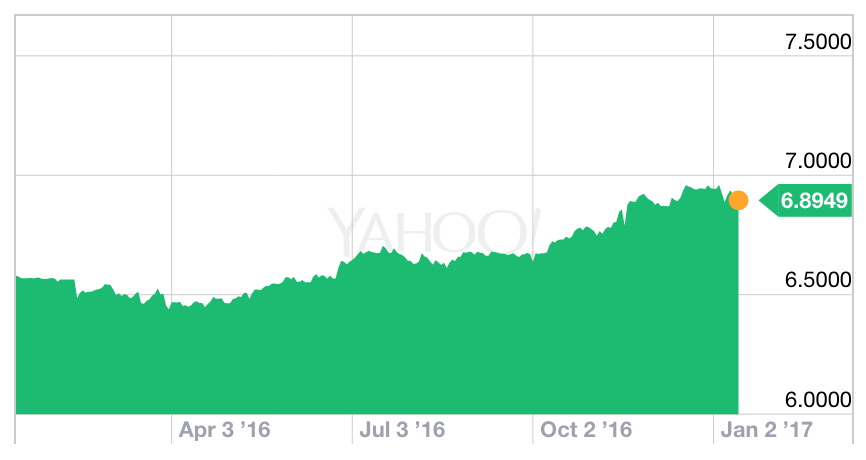
\includegraphics[width=.5\linewidth]{./Figure/USD-CNY.png}
\caption{USD to CNY exchange rate. Jan 12 2016 - Jan 12 2017. Source, Yahoo finance.}
\end{figure}

Given input of a stock price series, our system will first fit some powerful and popular time series models, such as autoregressive (AR) model, moving average (MA) model and other derived models. This procedure will give you the estimation of parameters in these models. 

The most important task in estimation is the optimization procedure. Users can select one of optimization methods in the system based on their preference. The optimization method includes but not limited to gradient descent and Newton’s method.

After model fitting and estimation, our system provides a fast way to do statistical inference. Users can do different kinds of statistical test as well as confidence interval. Moreover, with fitted model, future price prediction is made and it’s compared with real price data. Moreover, we provide different methods to assess the prediction accuracy, which will be visualized afterwards. With the identified model, we can further consider trading strategy and option pricing.

More interestingly, if users input multiple stock prices, we can divide these stocks into different groups, which is called clustering. Among each group, stocks share similarity. Different clusters will also be visualized. With collection of stocks (e.g., S\&P 500), we can exploit the correlations within them and build a reduced order model for price prediction. For example, principal component analysis can be used to extract dominant features in the finanical market.

\section{Design process}
We decide to use python, since it's free, and widely distributed. Moreover, there are many powerful packages, e.g., numpy, scipy, etc.

We make use of existing packages like numpy and matplot, but largely other parts are made by our group. For example, optimization method like gradient descent are implemented by us.

Github is used to track the progress of this project, and streamlines the colleboration within our group.

Along the way, we have adopted the philosiphy of object oriented programming (OOP) by carefully designing classes which include relevant functions.

Part of our code are tested using Python unittest, since there are analytical solutions. For more complicated functions, they are tested using canonical examples, and by comparing with the outputs of standard machine learning package scikit-learn.

Doxygen is used to document this project. Add explainations for doxygen.
\begin{figure}[H]
        \centering
     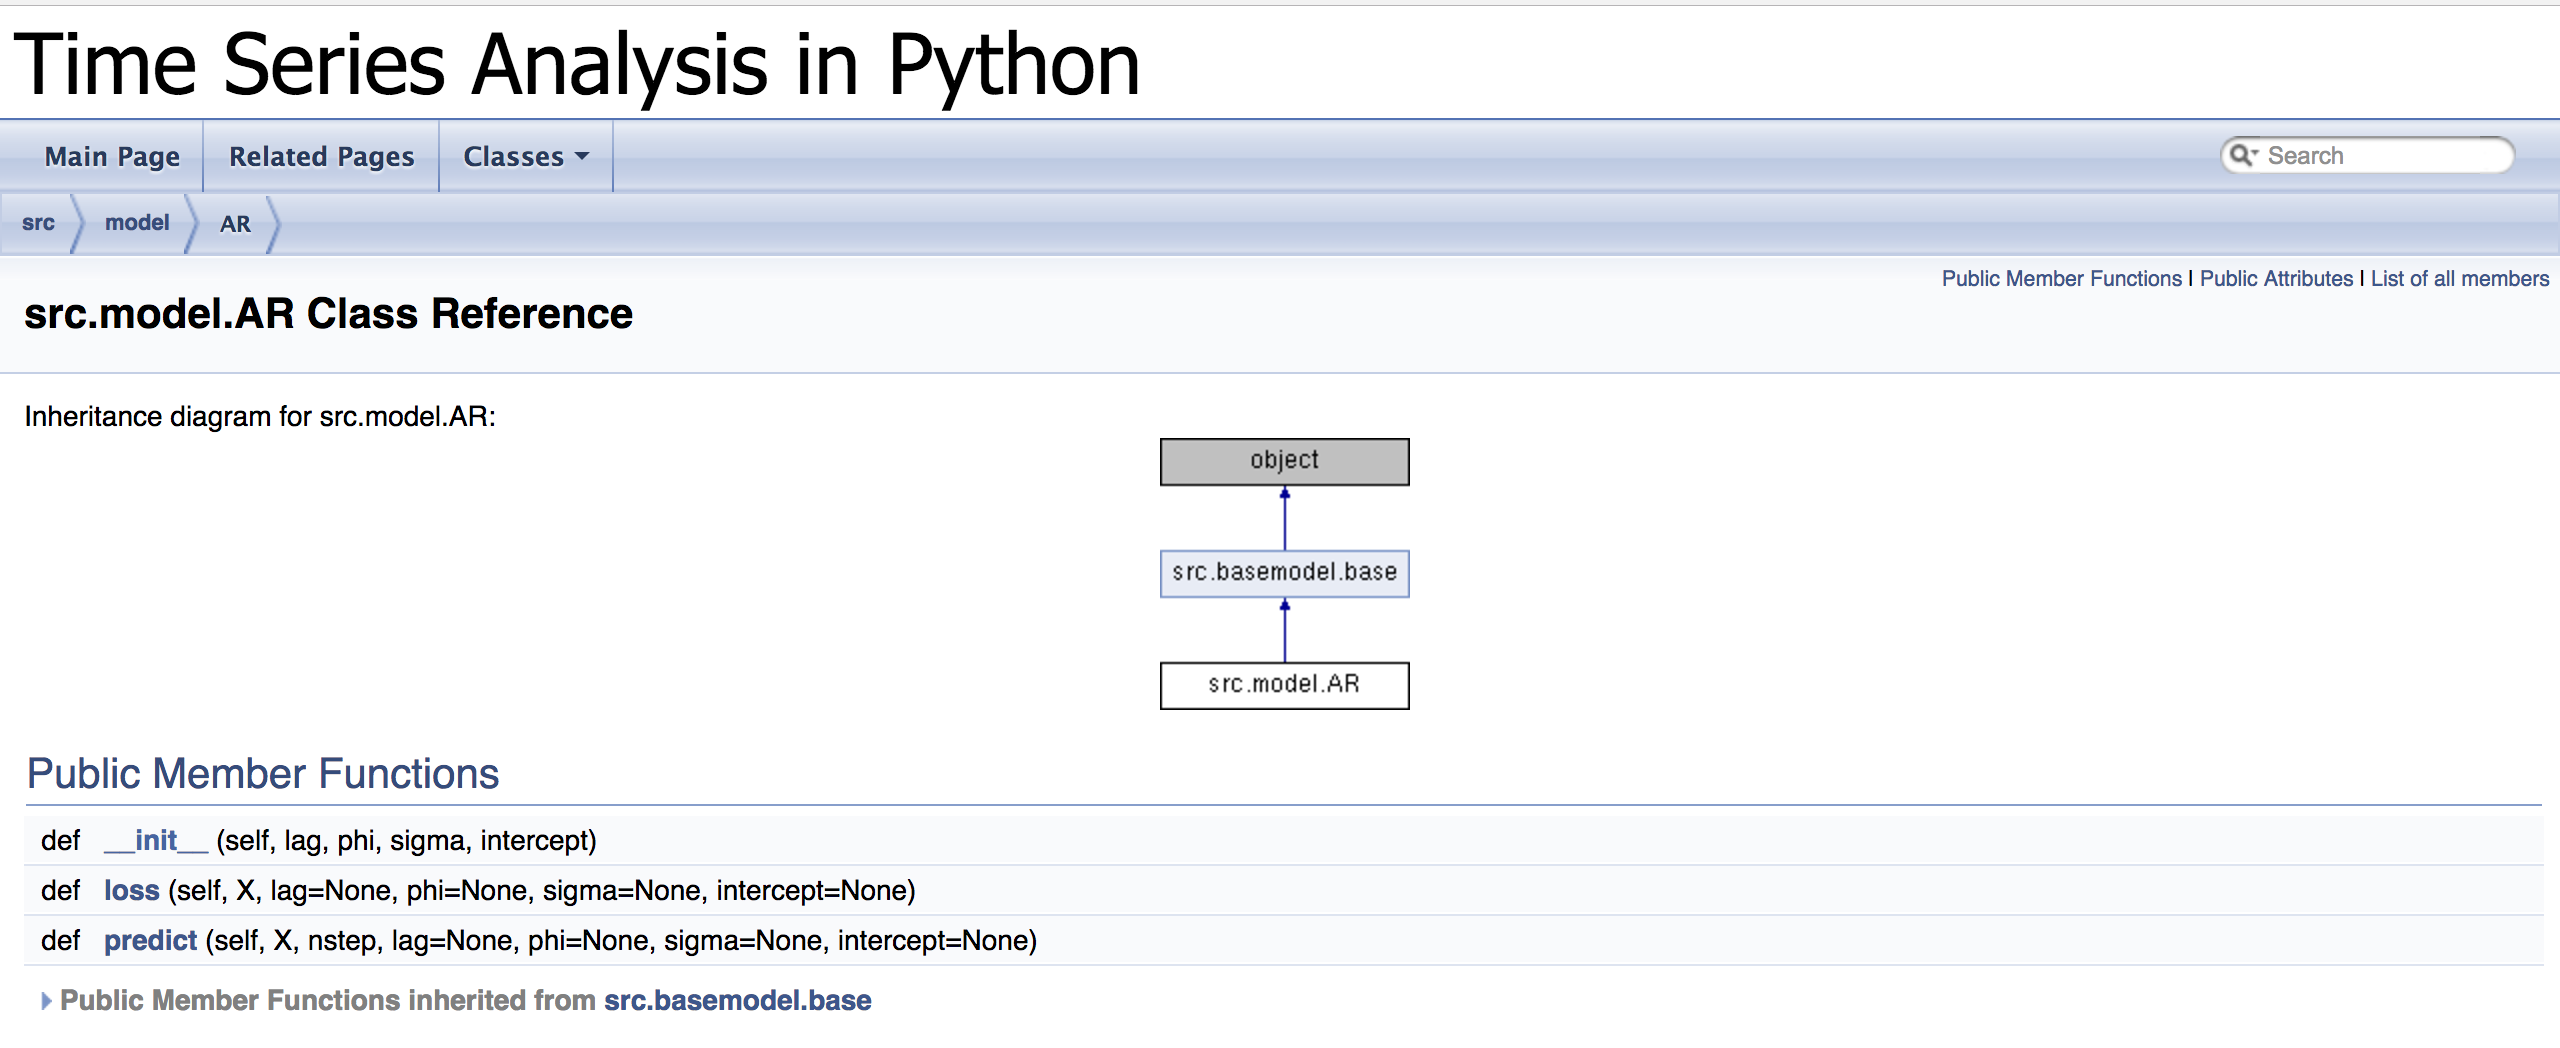
\includegraphics[width=.7\linewidth]{./Figure/Doxygen.png}
\caption{Doxygen documentation}
\end{figure}

We have a few milestones for this project. (1) Prototype, Dec 15. In this release, we had at least one implementation for each step. Then given a time series data, we could apply at least one method from each class to do the analysis. (2) Alpha version, Jan 1. In this release, we completed most methods in each class. (3) Final version, Jan 12.  In this relase, we finalized the project. Finish all the testing using various data including simulated data and real finanical data.

\section{Architecture}
The high-level program structure is shown below. The division of work is pretty even, and there are some minor work that are too trivial to mention extensively here. Overall, the program consists of two parts. The first part deal with a single time series, and exploits the time correlation within the time series. There is data preprocessing module that takes the raw data and get the right dataformat for later analysis. Optimization, model, and solver are used all together to identify the models. Finally, there is a post processing module that makes use of the information from model. The post processing module includes parameter inference, trading strategy, and option pricing. The second part deals with a collection of time series of data, basically it exploits the correlation between different time series. In this way, we can gain more insights into the finanical market. While these insights are impossible for a single time series.
\begin{figure}[H]
        \centering
     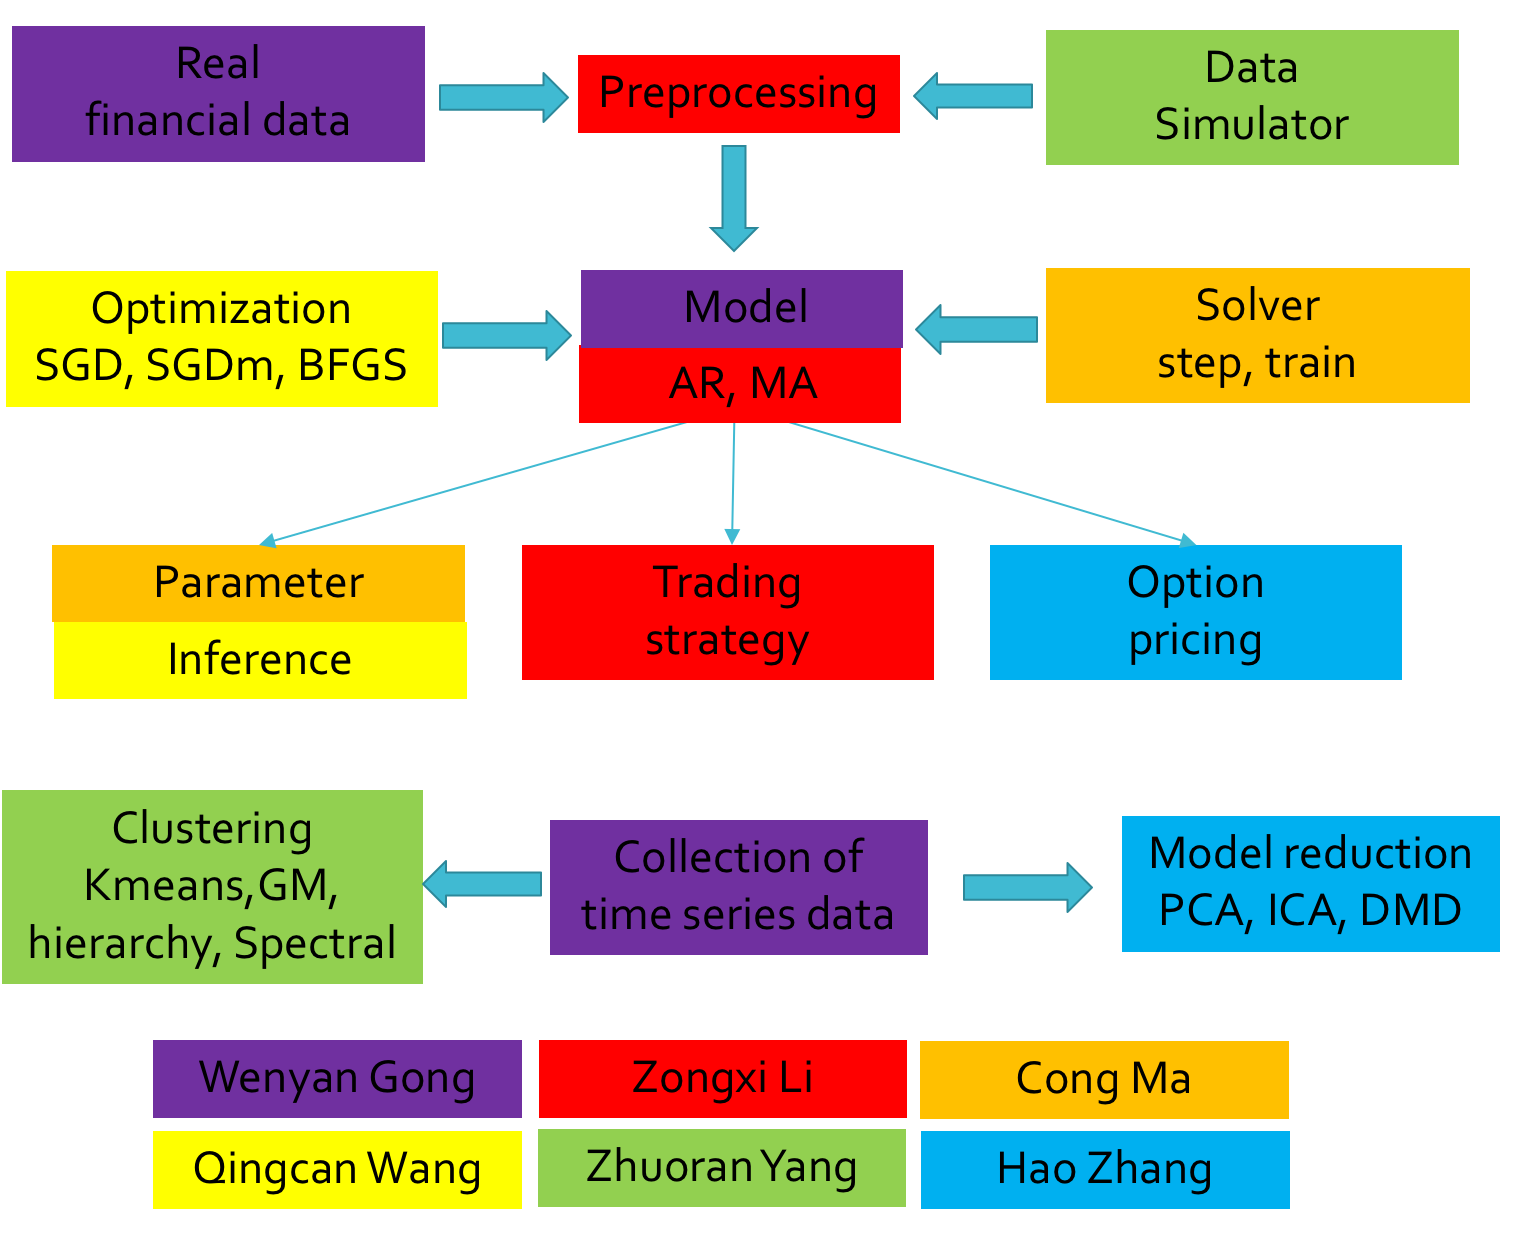
\includegraphics[width=.5\linewidth]{./Figure/structure.png}
\caption{Program structure and division of work}
\end{figure}

\subsection{Data collection \& preprocessing}
We develop simulator to simulate data for model testing. At the same time, real finanical data (S\&P 500) are also collected from online source.

For the preprocessing part, we provide functions that can transfer the price time series to return time series and do the reverse transfering. For instance, if you input daily price of GOOGLE stock, then we can output the daily return of GOOGLE stock. If you input daily return of it, we can output the daily price. Moreover, we can detect the peak and trouph for a given time series, which will be used for developing trading strategy. For example, if you input GOOGLE stock price series, we can detect the highest price and the lowest price.

\subsection{Model}
For a given time serise, there are two kinds of model class that can be used to fit the time series. One is the autoregressive  (AR) model. The other is moving average (MA) model. Inside each class, we provide three functions, initialization, loss function and prediction function. 

To be specific, we can first initialize the model with given parameters. Secondly, the loss funtion is able to calculate return the current loss as well as gradient of negative loglikelihood function, based on the current parameters in the model. This is crutial, because the loss and gradient will be the input of the optimization method, which will in turn return the updated model for the loss function to calculte new loss and gradient. Finally, the prediction function is able to predict the future time series based on historical time series and fitted parameters.


\subsection{Optimization}
After the model type being fixed, there would be certain loss function regarding the selected model. The key of model fitting is to decide the parameters, which are derived by minimizing the loss function. Therefore, certain optimization techniques should be applied during the fitting. In our software, the user could choose the optimization tool between gradient descent, Newton method and stochastic gradient descent according to the scale of the problem.

\subsection{Solver}
We develop a solver module as the main driver program that uses both model and optimization method to find the solution. It allows the user to update the parameters in the model for one step each, and also allows the user to update them untill convergence.

\subsection{Inference}
After model fitting, in order to provide the user with more overall information about the model, our software also do inference work regarding the parameters. The software would construct confidence interval of given level for each parameter, conduct test to decide the non-zero parameters and calculate the corresponding P-value. This could help to identify the pattern of the model and help the user develop deeper understanding of the given time series.

\subsection{Trading strategy}

The software is able to generate trading signal based on predicted price. To be specific, it can detect which time point to buy and which to sell.  Moreover, it can calculate the profit and loss based on existing trading signal. 

The most important part is a function that can automatically do the trading with historical data and fitted model. This function will call other  functions from the "model" as well as the functions that generate signals and calculate the profit. It will finally return the predicted price, trading signal and profit time series. Moreover, there're many options for the trading, for instance, you can specify the trading frequency, the prediction length. 


\subsection{Option pricing}
option pricing

\subsection{Clustering}


\subsection{Model reduction}
model reduction

program structure, division of work, user interface, 
independent component analysis \cite{hyvarinen2000independent}.

\section{Demos of results}
\subsection{Modal validation}
\subsection{Finanical data}
\subsection{Trading strategy}
In this section, we demonstrate how we can use our code to do the trading strategy. We pick GOOGLE stock price from 01/02/2015 to 12/09/2016, which contains 490 trading days data. To begin with,  we made use of the first 100 data points to fit AR(5) model, and then predicted future prices. This part is similar to the above section, so we will omit the details, including the optimization procedure. After getting the fitted model, we input it as well as some parameters into trading package. There, we specify the parameters as follows. The training length $l=100$. The prediction step is $nstep=20$. The length of trading window $window=5$. And the initial money to invest $money=100$. 

\subsection{Option pricing}
\subsection{Clustering}
\subsection{Model reduction}

\section{Lessons learned}

\bibliography{ref}
\end{document}